\experiment{Problema inicial}

Se plantea realizar un montaje experimental de tres péndulos
rígidos acoplados, con el objetivo de modelar el sistema bajo
pequeñas oscilaciones, así como visualizar sus modos normales
y estudiar su movimiento asociado.

La \cref{fig:system-diagram} presenta la configuración inicial
del sistema, donde la longitud del péndulo central (\( \ell \))
es el doble de las otras dos. Los péndulos laterales están
separados por una distancia \( a \), y cuentan con 5 posibles
puntos de acople a lo largo del cuerpo rígido.

\begin{figure}[htbp!]
	\centering
	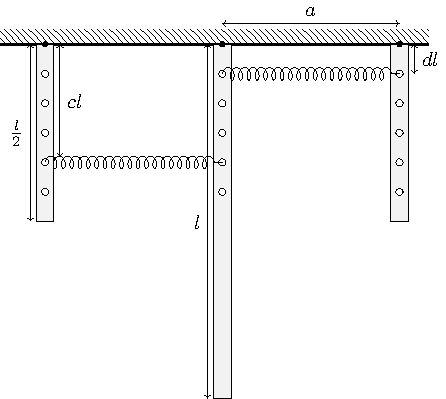
\includegraphics[width=0.75\linewidth]{./Figures/system-diagram.pdf}
	\caption{Configuración inicial del montaje experimental.}
	\label{fig:system-diagram}
\end{figure}

Se plantean los siguientes objetivos a desarrollar:

\begin{itemize}
	\item Desarrollar el modelo teórico que describe el sistema de
		tres péndulos rígidos acoplados bajo la aproximación de pequeñas
		oscilaciones, para determinar sus modos normales y frecuencias propias.
	\item Diseñar y construir un montaje experimental que permita la observación
		y caracterización de los modos normales.
	\item Recopilar los datos experimentales necesarios de las oscilaciones del
		sistema y analizarlos para identificar los modos normales observados,
		sus frecuencias asociadas y compararlos con las predicciones teóricas.
\end{itemize}
